\documentclass[12pt]{article}
\usepackage[margin=2.5cm]{geometry}
\usepackage{enumerate}
\usepackage{amsfonts}
\usepackage{amsmath}
\usepackage{fancyhdr}
\usepackage{amsmath}
\usepackage{amssymb}
\usepackage{amsthm}
\usepackage{mdframed}
\usepackage{graphicx}
\usepackage{subcaption}
\usepackage{adjustbox}
\usepackage{listings}
\usepackage{xcolor}
\usepackage{booktabs}
\usepackage[utf]{kotex}
\usepackage{hyperref}

\definecolor{codegreen}{rgb}{0,0.6,0}
\definecolor{codegray}{rgb}{0.5,0.5,0.5}
\definecolor{codepurple}{rgb}{0.58,0,0.82}
\definecolor{backcolour}{rgb}{0.95,0.95,0.92}

\lstdefinestyle{mystyle}{
    backgroundcolor=\color{backcolour},
    commentstyle=\color{codegreen},
    keywordstyle=\color{magenta},
    numberstyle=\tiny\color{codegray},
    stringstyle=\color{codepurple},
    basicstyle=\ttfamily\footnotesize,
    breakatwhitespace=false,
    breaklines=true,
    captionpos=b,
    keepspaces=true,
    numbers=left,
    numbersep=5pt,
    showspaces=false,
    showstringspaces=false,
    showtabs=false,
    tabsize=1
}

\lstset{style=mystyle}

\pagestyle{fancy}
\renewcommand{\headrulewidth}{0.4pt}
\lhead{Team Treehouse}
\rhead{Java Objects Part 1 Notes}

\begin{document}
\title{Java Objects Part 1 Notes}
\author{Team Treehouse}
\maketitle

\bigskip

\section{Welcome Back}

\bigskip

\begin{itemize}
    \item \textit{STRING.toLowerCase()}
    \begin{itemize}
        \item Turns string into lowercase letter
    \end{itemize}
    \item \textit{STRING.contains(...)}
    \begin{itemize}
        \item checks if value \textit{...} is contained inside \textit{String}
    \end{itemize}
\end{itemize}

\bigskip

\section{Quiz 1}

\bigskip

\begin{enumerate}[1.]
    \item

    Please fill in the correct answer in each blank provided below.

    \bigskip

    \begin{lstlisting}[language=Java]
    String someWords = "These are words";
    someWords.______("words");
    \end{lstlisting}

    \bigskip

    \textbf{Answer:}

    \bigskip

    \begin{lstlisting}[language=Java]
    String someWords = "These are words";
    someWords.contains("words");
    \end{lstlisting}

    \item

    The boolean datatype is used to store:

    \bigskip

    \begin{enumerate}[A.]
        \item numbers
        \item text
        \item true or false values
    \end{enumerate}

    \bigskip

    \textbf{Answer:} C

    \item Please fill in the correct answer in each blank provided below.

    \bigskip

    What operator do we use to ensure that both of these conditions are met:

    \begin{lstlisting}[language=Java]
    boolean isRefreshed = true;
    boolean isReadyToGetStarted = true;
    boolean shouldContinue = isRefreshed______isReadyToGetStarted;
    \end{lstlisting}

    \bigskip

    \textbf{Answer:}

    \bigskip

    \begin{lstlisting}[language=Java]
    boolean isRefreshed = true;
    boolean isReadyToGetStarted = true;
    boolean shouldContinue = isRefreshed && isReadyToGetStarted;
    \end{lstlisting}


    \item Please fill in the correct answer in each blank provided below.

    \bigskip

    \begin{lstlisting}[language=Java]
    int weightOfCraigsKid = 50;
    int weightMonty = 130;
    if (weightMonty ______ weightOfCraigsKid) {
        console.printf("Whoa that's a huge dog!");
    }
    \end{lstlisting}

    \bigskip

    \textbf{Answer:}

    \bigskip

    \begin{lstlisting}[language=Java]
    int weightOfCraigsKid = 50;
    int weightMonty = 130;
    if (weightMonty > weightOfCraigsKid) {
        console.printf("Whoa that's a huge dog!");
    }
    \end{lstlisting}

    \item To define a new variable to store a name it would look something like
    this:

    \bigskip

    \begin{enumerate}[A.]
        \item String firstName = "Bob";
        \item "Bob" = first.name
        \item firstName = "Bob";
        \item first\_name = 'Bob'
    \end{enumerate}

    \bigskip

    \textbf{Answer:} A

    \item The boolean datatype is used to store:

    \bigskip

    \begin{enumerate}[A.]
        \item numbers
        \item text
        \item true or false values
    \end{enumerate}

    \bigskip

    \textbf{Answer:} C

\end{enumerate}

\bigskip

\section{Creating Classes}

\bigskip

\begin{itemize}
    \item

    \begin{lstlisting}[language=Java,caption={lesson\_3/PezDispenser.java}]
    class PezDispenser {  // <- 1. Class is created in a separate and matching file :)
        String characterName = "Yoda";
    }
    \end{lstlisting}

    \bigskip

    \begin{lstlisting}[language=Java,caption={lesson\_3/Example.java}]
    import java.io.Console;

    public class Example {
        public static void main(String[] args) {

            System.out.println("We are making a new PEZ dispenser");

            PezDispenser dispenser = new PezDispenser(); // <- 2. And is used here :)

            System.out.printf("The dispenser is %s", dispenser.characterName);
            ...
        }
    }
    \end{lstlisting}
\end{itemize}

\bigskip

\section{Exercise 1}

\bigskip

\begin{itemize}
    \item Solution included in \textit{exercise\_1.java}
\end{itemize}

\bigskip

\section{Access Modifiers}

\bigskip

\begin{center}
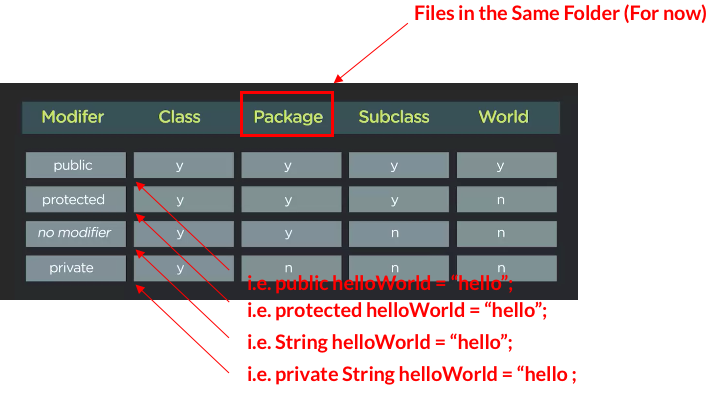
\includegraphics[width=\linewidth]{images/part_1_notes_1.png}
\end{center}

\begin{itemize}
    \item Determines who is intended to access the information
    \item Adding access modifiers to attributes and methods in class is called
    \textbf{Encapsulation}

    \begin{lstlisting}[language=Java,caption={lesson\_5/PezDispenser.java}]
    class PezDispenser {
        private String characterName = "Yoda"; // <- 1. attribute is turned private
    }
    \end{lstlisting}

    \bigskip

    \begin{lstlisting}[language=Java,caption={lesson\_5/Example.java}]
    import java.io.Console;

    public class Example {
        public static void main(String[] args) {

            System.out.println("We are making a new PEZ dispenser");

            PezDispenser dispenser = new PezDispenser();

            System.out.printf("The dispenser is %s", dispenser.characterName); // <- 2. and it can't be accessed outside of class
        }
    }
    \end{lstlisting}

    \bigskip

    \underline{\textbf{Notes:}}

    \bigskip

    \begin{itemize}
        \item Files can be compiled and displayed by typing \textit{javac Example.java \&\& java Example}
        in terminal
    \end{itemize}
\end{itemize}

\bigskip

\section{Exercise 2}

\bigskip

\begin{itemize}
    \item Solution included in \textit{exercise\_2.java}
\end{itemize}

\bigskip

\section{Methods}

\bigskip

\begin{itemize}
    \item is a collection of statements that are grouped together to perform an
    operation
    \item is like \textit{verb}
    \item \textit{ACCESS\_MODIFIER DATA\_TYPE get\textless ATTRIBUTE\_NAME \textgreater}
    is called \textbf{getter}
\end{itemize}

\bigskip

    \begin{lstlisting}[language=Java,caption={lesson\_7/PezDispenser.java}]
    public class PezDispenser {
        private String characterName = "Yoda";

        public String getCharacterName() { // <- 1. Getter method added here
            return characterName;
        }
    }
    \end{lstlisting}

    \bigskip

    \begin{lstlisting}[language=Java,caption={lesson\_7/Example.java}]
    import java.io.Console;

    public class Example {
        public static void main(String[] args) {

            System.out.println("We are making a new PEZ dispenser");

            PezDispenser dispenser = new PezDispenser();

            System.out.printf("The dispenser is %s", dispenser.getCharacterName()); // <- 2. And is used here
        }
    }
    \end{lstlisting}

\bigskip

\section{Exercise 3}

\bigskip

\begin{itemize}
    \item Solution included in \textit{exercise\_3.java}
\end{itemize}

\bigskip

\section{Constructors}

\bigskip

\begin{itemize}
    \item is a method that will run when class is instantiated.
    \item is created by writing a method with the same name as class
    \item \textit{this} is like \textit{self} in python
\end{itemize}


    \begin{lstlisting}[language=Java,caption={lesson\_9/PezDispenser.java}]
    public class PezDispenser {
        private String characterName = "Yoda";

        public PezDispenser(String characterName) {
            this.characterName = characterName;
        }

        public String getCharacterName() {
            return characterName;
        }
    }
    \end{lstlisting}

    \bigskip

    \begin{lstlisting}[language=Java,caption={lesson\_9/Example.java}]
    import java.io.Console;

    public class Example {
        public static void main(String[] args) {

            System.out.println("We are making a new PEZ dispenser");

            PezDispenser dispenser = new PezDispenser("Yoda");

            System.out.printf("The dispenser is %s", dispenser.getCharacterName()); // <- 2. And is used here
        }
    }
    \end{lstlisting}

\bigskip

\section{Exercise 4}

\bigskip

\begin{itemize}
    \item Solution included in \textit{exercise\_4.java}
\end{itemize}

\end{document}